%==============================================================================
%  ICCIT 2026 submission -- IEEE conference format, A4, 6 pages maximum.
%
%  DOUBLE-BLIND: ICCIT rejects manuscripts that carry author names,
%  affiliations, postal addresses or e-mail addresses. The author block below
%  is anonymised on purpose. Restore it only for the camera-ready version.
%  The same applies to the code repository link in Section VII.
%==============================================================================
\documentclass[conference,a4paper]{IEEEtran}
\IEEEoverridecommandlockouts

\usepackage{cite}
\usepackage{amsmath,amssymb}
\usepackage{graphicx}
\usepackage{booktabs}
\usepackage{url}
\usepackage{pgfplots}
\pgfplotsset{compat=1.18}

\def\BibTeX{{\rm B\kern-.05em{\sc i\kern-.025em b}\kern-.08em T\kern-.1667em\lower.7ex\hbox{E}\kern-.125emX}}

\begin{document}

\title{When Is Short-Term PM$_{2.5}$ Forecasting Actually Possible?\\
Horizon-Dependent Skill and Evaluation Leakage\\
Across Twelve Cities}

% --- ANONYMISED FOR DOUBLE-BLIND REVIEW ------------------------------------
% For the camera-ready version, replace this block with the real author list.
\author{\IEEEauthorblockN{Anonymous Submission}
\IEEEauthorblockA{Paper ID: XXXX}}
% ---------------------------------------------------------------------------

\maketitle

\begin{abstract}
Machine-learning models for short-term PM$_{2.5}$ forecasting are routinely
reported with coefficients of determination above $0.95$, yet the naive forecast
that tomorrow's pollution equals today's is rarely used as a reference. We
evaluate one-hour-ahead PM$_{2.5}$ prediction against a persistence baseline on
nine years of hourly data from the U.S. Embassy monitor in Dhaka, and find that a
gradient-boosted ensemble is not statistically distinguishable from persistence
(skill $3.4\%$, $p=0.10$). Forecast skill is strongly horizon-dependent: it rises
to $40.0\%$ at twelve hours ahead ($p<10^{-4}$, standard deviation $0.1\%$ across
seeds) before declining again. We then quantify two evaluation practices common
in this literature. Holding the test set constant, random rather than
chronological splitting reduces error by $0.8\%$ and is not significant
($p=0.31$); including the same-hour NowCast concentration, a smoothed function of
the target, reduces error by $19.9\%$ ($p<10^{-4}$). Replicating both experiments
across twelve cities on five continents drawn from a single monitoring programme,
the horizon effect holds in $12$ of $12$ cities and the NowCast inflation in $12$
of $12$, with a median of $42.5\%$. In $7$ of $12$ cities that inflation exceeds
the entire genuine skill available at any horizon. We argue that reporting a
persistence baseline and an explicit feature-timing statement should be minimum
practice for this class of work.
\end{abstract}

\begin{IEEEkeywords}
air quality forecasting, PM$_{2.5}$, data leakage, forecast skill, evaluation
methodology, persistence baseline
\end{IEEEkeywords}

%==============================================================================
\section{Introduction}
%==============================================================================

Dhaka has among the highest recorded fine-particulate concentrations of any
capital city. In the record analysed here the median hour sits at
$65~\mu\mathrm{g/m^3}$, more than four times the World Health Organization
24-hour guideline, and the worst hour reaches $985~\mu\mathrm{g/m^3}$. A reliable
short-term forecast would let schools, hospitals and outdoor workers act before a
pollution episode rather than during it.

A large literature applies machine learning to this problem, and a substantial
part of it reports performance that is difficult to reconcile with the physical
variability of the series. One recent study of Dhaka reports $R^2 = 0.998$ with
$\mathrm{RMSE} = 3.07~\mu\mathrm{g/m^3}$ from temporal features alone
\cite{dhaka_compare}. On the same station, simply repeating the previous hour's reading
yields $\mathrm{RMSE} \approx 35~\mu\mathrm{g/m^3}$, and the hour-to-hour change
has a standard deviation of $33.2~\mu\mathrm{g/m^3}$. Predicting to within
$3~\mu\mathrm{g/m^3}$ would require near-perfect anticipation of a quantity that
routinely moves by an order of magnitude more.

Two explanations are available, and both are measurable. The first is that the
evaluation split does not respect time, allowing a model to be trained on hours
adjacent to those it is tested on. The second is that a feature available at
prediction time in the dataset would not be available at prediction time in
deployment. Neither is detectable from reported metrics alone; both are
invisible unless the paper states its split strategy and its feature timing.

This paper makes three contributions.

\begin{enumerate}
\item \textbf{A horizon-dependent skill curve.} One hour ahead, a tuned ensemble
      is statistically indistinguishable from persistence. Skill rises with
      horizon to $40.0\%$ at twelve hours and declines thereafter. The result is
      stable across four rolling-origin folds and five random seeds.
\item \textbf{A controlled quantification of two evaluation shortcuts.} On a
      single shared test set with significance testing, random splitting
      contributes $0.8\%$ ($p=0.31$, not significant) while same-hour smoothed
      concentration contributes $19.9\%$ ($p<10^{-4}$).
\item \textbf{A twelve-city replication.} Both effects are tested on twelve
      cities across five continents drawn from a single monitoring programme
      with a common instrument and quality-control procedure. The horizon effect
      holds in $12/12$ cities; the leakage effect holds in $12/12$ with a median
      of $42.5\%$, and in $7/12$ exceeds the best genuine skill available.
\end{enumerate}

%==============================================================================
\section{Related Work}
%==============================================================================

\subsection{PM$_{2.5}$ prediction in South Asia}
Comparative studies of PM$_{2.5}$ prediction for Dhaka and neighbouring cities
have appeared regularly, typically evaluating Random Forest, XGBoost, CatBoost
and LSTM on multi-year hourly records \cite{dhaka_compare,dhaka_health}. These
studies report $R^2$ and RMSE and rank the models against one another. Rankings
of this kind establish which estimator fits best; they do not establish whether
any of them carries information beyond the autocorrelation of the series, which
requires a reference forecast.

\subsection{Reference forecasts and forecast skill}
A forecast that cannot outperform a method using little or no problem-specific
information has no skill \cite{forecast_review}. Persistence and seasonal-naive
forecasts quantify how much apparent performance follows from autocorrelation and
recurring cycles alone, and a recent systematic mapping review of over four
hundred air-quality forecasting studies recommends establishing them before
introducing deep or spatial structure \cite{forecast_review}. Our finding at
short horizons agrees with a recent continuous-time neural model, which reported
near-zero skill scores at short lead times and attributed them to the
predictability limit of the pollutant in the absence of meteorological drivers
\cite{manode}.

\subsection{Leakage in machine-learning-based science}
Leakage has been documented across seventeen scientific fields, affecting
hundreds of papers and in several cases producing conclusions that did not
survive re-analysis \cite{kapoor}. Random partitioning of a time series is the
canonical instance: it allows information from the future into training and
inflates every metric. Reporting standards have been proposed in response
\cite{reforms}, and realistic evaluation benchmarks have begun to appear for air
quality specifically \cite{aqbench}. The present work differs in measuring the
size of two specific effects, under controlled conditions, on the data where
they would occur.

%==============================================================================
\section{Data}
%==============================================================================

\subsection{Source}
All data come from the AirNow Department of State programme, which operated
reference-grade PM$_{2.5}$ monitors at more than eighty U.S. embassies and
consulates and published hourly measurements in a common format. The programme
was defunded in March 2025 and public reporting ceased; a subsequent study
reported satellite-measured pollution increases of $24$--$33\%$ across
forty-six cities in the months that followed \cite{shutdown}.

Using a single programme rather than an aggregation of national networks is a
deliberate methodological choice. Comparing cities across monitoring networks
would confound differences in the air with differences in instrumentation,
calibration schedules and quality-control procedure. Here the instrument, the
file format and the quality-control field are common to every city, so the
principal variable across sites is the atmosphere itself.

\subsection{Coverage}
Nineteen cities have complete PM$_{2.5}$ records for 2016--2024; twelve were
selected to span the observed concentration range and five continents
(Table~\ref{tab:cities}). The Dhaka record used for the detailed analysis runs
from 2016-03-01 to 2025-03-24 and contains $77{,}716$ rows.

\subsection{Quality characteristics}
Profiling the Dhaka record before modelling identified five properties that
affect the construction of any supervised dataset from it.

\begin{itemize}
\item \textbf{Non-valid rows.} $2{,}342$ of $77{,}716$ rows carry a
      quality-control flag of \texttt{Missing}, \texttt{Invalid} or
      \texttt{Suspect} together with a sentinel value of $-999$. A further
      $94$ rows are flagged valid yet retain the sentinel in the NowCast field.
\item \textbf{Missing hours.} $4{,}089$ hours ($5.1\%$) are absent across $517$
      separate gaps. $419$ gaps are a single hour; the longest is $1{,}822$
      hours (76 days, August--November 2018).
\item \textbf{Duplicated hours.} Six timestamps appear twice with differing
      readings. Four fall on the second Sunday in March of consecutive years,
      the date of the United States daylight-saving transition, indicating that
      the export process operated on a US clock.
\item \textbf{Physically impossible values.} $24$ readings are negative, the
      lowest $-4.0~\mu\mathrm{g/m^3}$.
\item \textbf{Distributional shape.} Skewness is $+1.863$; under a
      $\log(1+x)$ transform it is $-0.245$.
\end{itemize}

\begin{table}[t]
\caption{Cities analysed. All records are 2016--2024 from a single monitoring
programme. Rows are usable hours after preprocessing.}
\label{tab:cities}
\centering
\small
\begin{tabular}{@{}lrrr@{}}
\toprule
City & Usable rows & Mean PM$_{2.5}$ & Region \\
     &             & ($\mu$g/m$^3$)  &        \\
\midrule
New Delhi        & 73{,}064 & 101.2 & South Asia \\
Dhaka            & 69{,}927 &  97.7 & South Asia \\
Kolkata          & 67{,}126 &  69.8 & South Asia \\
Ulaanbaatar      & 56{,}060 &  45.5 & East Asia \\
Hanoi            & 61{,}769 &  43.9 & Southeast Asia \\
Beijing          & 75{,}194 &  43.3 & East Asia \\
Mumbai           & 65{,}893 &  43.1 & South Asia \\
Chennai          & 66{,}117 &  30.8 & South Asia \\
Jakarta (Central)& 73{,}249 &  30.5 & Southeast Asia \\
Shanghai         & 62{,}155 &  26.0 & East Asia \\
Addis Ababa      & 56{,}461 &  20.4 & Africa \\
Bogot\'a         & 61{,}935 &  17.3 & South America \\
\bottomrule
\end{tabular}
\end{table}

%==============================================================================
\section{Method}
%==============================================================================

\subsection{Reconstructing a gap-free hourly index}
Lag features are conventionally computed with a row-offset window function. Where
hours are missing, a row offset and an hour offset are not the same quantity: at
the boundary of the 76-day gap, the previous row is 76 days earlier while being
labelled as the previous hour.

We therefore generate every hour between the first and last observation
($79{,}457$ hours) and left-join the observations onto that index, so missing
hours become explicit null rows rather than silent absences. A one-row-per-hour
assertion is checked before any feature is computed. All lag and lead operations
are performed on this complete index, before any subsequent filtering.

Duplicated hours are collapsed by averaging rather than by arbitrary selection,
since the duplicated readings differ and an arbitrary choice would not be
reproducible between runs. Negative readings are clipped to zero rather than
deleted, to avoid creating further gaps.

\subsection{Features}
Fourteen predictors are derived exclusively from hours strictly preceding the
target: lagged concentrations at $1$, $2$, $3$ and $24$ hours; rolling mean over
$3$ and $24$ hours and rolling standard deviation over $24$ hours, all windows
terminating at $t-1$; the NowCast value lagged by one hour; and calendar terms
for hour and month, each additionally encoded as a sine--cosine pair so that
hour $23$ and hour $0$ are adjacent.

Lag selection follows the autocorrelation structure of the series, which falls
monotonically to $0.545$ at twelve hours and then rises to $0.725$ at
twenty-four, reflecting the diurnal cycle (Fig.~\ref{fig:acf}).

Rolling statistics are computed over whatever hours are available rather than
requiring a complete window. To prevent a 24-hour mean being computed from three
observations, rows with fewer than $20$ of the preceding $24$ hours present are
excluded. The count itself is used as a gate and not as a predictor, since its
distribution differs between periods ($88.7\%$ complete windows in the training
years against $97.0\%$ in the test years) and therefore encodes instrument
availability rather than atmospheric state.

\subsection{Excluded variables}
The dataset provides a NowCast concentration and an air quality index for every
hour. NowCast is a weighted average over approximately the preceding twelve
hours \emph{inclusive of the current hour}, and the index is derived from it.
Same-hour correlations with the target are $0.975$ and $0.937$ respectively.
Both are excluded from the predictor set; only their lagged values are admitted.
Section~\ref{sec:leak} measures what their inclusion would buy.

\subsection{Evaluation protocol}
Data are partitioned chronologically into training (2016-03 to 2022-12,
$53{,}445$ rows), validation (2023, $8{,}622$ rows) and test (2024-01 to 2025-03,
$10{,}655$ rows). Pairwise timestamp intersections are verified empty. All model
and feature selection is performed on the validation partition; the test
partition is evaluated once.

Performance is reported as skill relative to persistence,
\begin{equation}
S = 1 - \frac{\mathrm{RMSE}_{\text{model}}}{\mathrm{RMSE}_{\text{persistence}}},
\end{equation}
where the persistence forecast at any horizon is the most recent observed value.
Differences between forecasts are tested with the Diebold--Mariano statistic
\cite{dm} on squared-error differentials, using a Newey--West
heteroskedasticity- and autocorrelation-consistent variance \cite{nw} and the
Harvey--Leybourne--Newbold small-sample correction \cite{hln}. Because
neighbouring forecast errors are correlated and the forecasts are demonstrably
not optimal, results are reported under both the theoretical bandwidth $h-1$ and
a wider data-driven bandwidth $\lfloor n^{1/3}\rfloor$; conclusions are reported
only where both agree.

The estimator is a random forest \cite{breiman} ($80$ trees, maximum depth $10$)
selected on validation over gradient-boosted trees and over a log-transformed
target. Implementation uses Apache Spark MLlib; all randomness is seeded.

%==============================================================================
\section{Results}
%==============================================================================

\subsection{One hour ahead}
On the Dhaka test partition the selected model attains
$\mathrm{RMSE} = 34.76~\mu\mathrm{g/m^3}$ against a persistence baseline of
$35.58$, a skill of $2.3\%$; on the shared-test-set configuration of
Section~\ref{sec:leak} the corresponding figures are $34.37$ and $35.58$, a skill
of $3.4\%$. The Diebold--Mariano statistic is $-1.64$ with $p=0.18$ under the
theoretical bandwidth and $p=0.10$ under the wider one. The improvement is not
statistically distinguishable from zero.

The coefficient of determination for this model is $0.854$. Persistence alone
achieves approximately $0.85$ on the same partition. An $R^2$ near $0.85$ is therefore
attainable on this series without any model at all, which is the principal reason
we report skill rather than $R^2$.

Feature importance is dominated by the one-hour lag at $0.70$; the next largest
contribution is the twenty-four-hour lag at $0.048$. The model is, to a first
approximation, reproducing the previous observation with small corrections.

\begin{figure}[t]
\centering
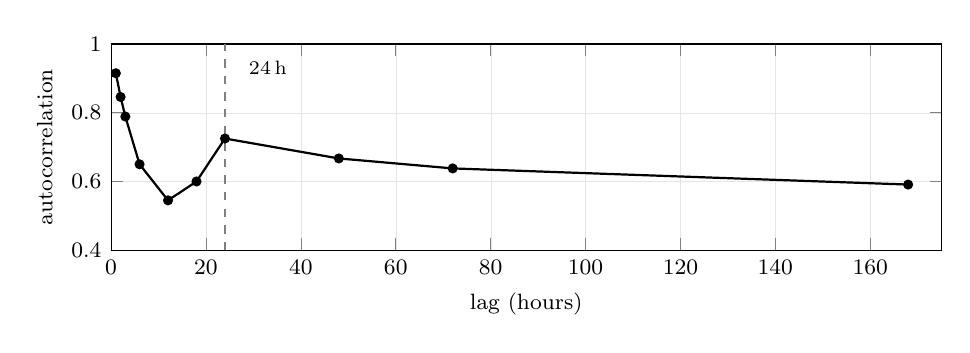
\begin{tikzpicture}
\begin{axis}[
  width=\columnwidth, height=4.2cm,
  xlabel={lag (hours)}, ylabel={autocorrelation},
  xmin=0, xmax=175, ymin=0.4, ymax=1.0,
  grid=both, grid style={line width=.1pt, draw=gray!20},
  tick label style={font=\footnotesize},
  label style={font=\footnotesize},
  mark size=1.4pt,
]
\addplot[thick, mark=*] coordinates {
  (1,0.915) (2,0.846) (3,0.789) (6,0.650) (12,0.545)
  (18,0.600) (24,0.725) (48,0.667) (72,0.638) (168,0.591)
};
\draw[dashed, gray] (axis cs:24,0.4) -- (axis cs:24,1.0);
\node[font=\scriptsize, anchor=west] at (axis cs:27,0.93) {24\,h};
\end{axis}
\end{tikzpicture}
\caption{Autocorrelation of hourly PM$_{2.5}$ in Dhaka. The minimum at twelve
hours and the recovery at twenty-four reflect the diurnal cycle and motivate the
choice of lags.}
\label{fig:acf}
\end{figure}

\subsection{Skill is horizon-dependent}
Table~\ref{tab:horizon} reports the same model and features at five forecast
horizons. Persistence error grows from $35.58$ to $93.82~\mu\mathrm{g/m^3}$
between one and twelve hours, while model error grows only from $34.37$ to
$56.33$. Skill rises to $40.0\%$ at twelve hours and is significant at
$p<10^{-4}$ under both bandwidths from three hours onward. Repeating the
twelve-hour configuration over five random seeds gives a mean skill of $39.9\%$
with a standard deviation of $0.1\%$.

The decline at twenty-four hours is a property of the reference rather than the
model: persistence itself improves at that horizon, from $93.82$ to $71.68$,
because the diurnal cycle returns the series toward its earlier value. Model
error is essentially unchanged between the two horizons.

Rolling-origin evaluation at one hour, training on all data preceding each of
2021--2024 and testing on that year, gives skills of $6.6\%$, $5.9\%$, $6.1\%$
and $6.0\%$: positive in every fold, with a standard deviation of $0.3\%$. A
seasonal-naive reference (the same hour on the previous day) gives
$\mathrm{RMSE} = 71.79$ at one hour and is not competitive with persistence at
that horizon.

\begin{table}[t]
\caption{Forecast skill against horizon, Dhaka test partition. $p$-values are
Newey--West corrected under the wider bandwidth; results under the theoretical
bandwidth agree throughout.}
\label{tab:horizon}
\centering
\small
\begin{tabular}{@{}rrrrrr@{}}
\toprule
Horizon & Persistence & Model & Skill & DM & $p$ \\
        & RMSE        & RMSE  &       &    &     \\
\midrule
1\,h  & 35.58 & 34.37 &  3.4\% &  $-1.64$ & 0.101 \\
3\,h  & 59.00 & 46.53 & 21.1\% &  $-7.75$ & $<10^{-4}$ \\
6\,h  & 78.70 & 53.26 & 32.3\% & $-10.82$ & $<10^{-4}$ \\
12\,h & 93.82 & 56.33 & \textbf{40.0\%} & $-10.92$ & $<10^{-4}$ \\
24\,h & 71.68 & 56.96 & 20.5\% &  $-5.86$ & $<10^{-4}$ \\
\bottomrule
\end{tabular}
\end{table}

\subsection{Two evaluation shortcuts, measured}
\label{sec:leak}
We train one estimator with identical settings under four conditions, varying
only the partitioning strategy and the admitted feature set. To ensure the
comparison is not confounded by test-set composition, the hold-out is assigned by
hashing the timestamp so that both feature sets withhold identical hours, and all
four conditions are evaluated on the intersection of the chronological test
period and the random hold-out: $1{,}567$ hours no condition trained on.

Table~\ref{tab:leak} reports the result. Random splitting reduces error by
$0.27~\mu\mathrm{g/m^3}$, $0.8\%$, which the Diebold--Mariano test does not
distinguish from zero ($p=0.31$). The same test resolves the other two conditions
at $\mathrm{DM}=4.16$ and $6.60$ on the same hours, so the null for random
splitting is not attributable to insufficient power. Admitting the same-hour
NowCast and index reduces error by $19.9\%$ ($p<10^{-4}$); admitting both
shortcuts reduces it by $32.7\%$.

We note that even both shortcuts together reach $R^2 = 0.933$, short of the
$0.998$ that motivated this investigation. They are therefore a partial rather
than a complete account of such figures.

\begin{table}[t]
\caption{Leakage audit. One estimator, four conditions, all evaluated on the
same $1{,}567$ hours. Gap is relative to condition A.}
\label{tab:leak}
\centering
\small
\begin{tabular}{@{}llrrrr@{}}
\toprule
 & Condition & RMSE & $R^2$ & Gap & $p$ \\
\midrule
A & chronological, honest & 35.02 & 0.851 & --- & --- \\
B & \textbf{random} split, honest & 34.74 & 0.854 & 0.27 & 0.307 \\
C & chronological, \textbf{leaky} & 28.06 & 0.904 & 6.95 & $<10^{-4}$ \\
D & \textbf{random} split, \textbf{leaky} & 23.56 & 0.933 & 11.46 & $<10^{-4}$ \\
\bottomrule
\end{tabular}
\end{table}

\subsection{Replication across twelve cities}
Both experiments were repeated on the twelve cities of Table~\ref{tab:cities}
using an identical pipeline and identical hyperparameters, with a chronological
split at 2024-01-01. Table~\ref{tab:cities_res} and Fig.~\ref{fig:cities} report
the outcome.

Twelve-hour skill exceeds one-hour skill in $12$ of $12$ cities. Under a null
hypothesis of no systematic difference this corresponds to a sign test at
$p \approx 5\times10^{-4}$. One-hour skill has a median of $4.9\%$ and is
\emph{negative} in four cities, where the fitted model is less accurate than
persistence. Twelve-hour skill has a median of $27.0\%$ and a minimum of
$15.0\%$.

The NowCast inflation is positive in $12$ of $12$ cities, with a median of
$42.5\%$ and a range of $2.7\%$ to $67.4\%$. Dhaka, at $23.1\%$, lies near the
low end of that range; had the study been conducted on Jakarta or Shanghai the
effect would have appeared two to three times larger. In $7$ of $12$ cities the
inflation exceeds the genuine twelve-hour skill for the same city.

A regional pattern is visible and we do not offer a verified mechanism for it:
the five South Asian cities show inflation between $2.7\%$ and $23.1\%$, while
all seven remaining cities fall between $40.8\%$ and $67.4\%$. Mean concentration
alone does not account for the split, since Chennai has the lowest inflation of
all twelve at a mid-range concentration.

\begin{table}[t]
\caption{Twelve-city replication. Skill is relative to persistence; inflation is
the error reduction obtained by admitting same-hour NowCast and index.}
\label{tab:cities_res}
\centering
\small
\begin{tabular}{@{}lrrr@{}}
\toprule
City & Skill 1\,h & Skill 12\,h & Inflation \\
\midrule
Dhaka             &   5.4\% & \textbf{40.8\%} & 23.1\% \\
Kolkata           &   4.3\% & 39.6\% & 17.8\% \\
Ulaanbaatar       &  11.5\% & 32.5\% & 45.7\% \\
Jakarta (Central) &   4.2\% & 30.7\% & \textbf{67.4\%} \\
Bogot\'a          &  12.7\% & 29.3\% & 46.1\% \\
Addis Ababa       &   8.5\% & 27.9\% & 44.2\% \\
New Delhi         & $-11.9\%$ & 26.1\% & 15.6\% \\
Mumbai            &  17.1\% & 25.3\% & 22.4\% \\
Chennai           & $-10.6\%$ & 25.2\% &  2.7\% \\
Hanoi             &   6.0\% & 21.1\% & 48.8\% \\
Shanghai          &  $-1.4\%$ & 16.9\% & 57.1\% \\
Beijing           &  $-0.4\%$ & 15.0\% & 40.8\% \\
\midrule
Median            &   4.9\% & 27.0\% & 42.5\% \\
\bottomrule
\end{tabular}
\end{table}

\begin{figure}[t]
\centering
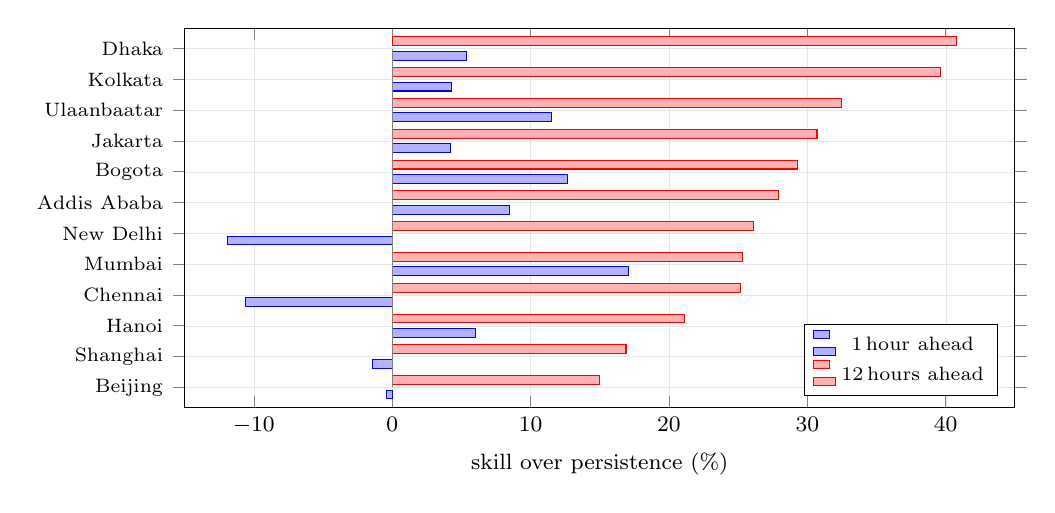
\begin{tikzpicture}
\begin{axis}[
  width=\columnwidth, height=6.4cm,
  xbar, bar width=3.2pt,
  xlabel={skill over persistence (\%)},
  xmin=-15, xmax=45,
  symbolic y coords={Beijing,Shanghai,Hanoi,Chennai,Mumbai,{New Delhi},
                     {Addis Ababa},{Bogota},{Jakarta},Ulaanbaatar,Kolkata,Dhaka},
  ytick=data,
  y tick label style={font=\scriptsize},
  tick label style={font=\footnotesize},
  label style={font=\footnotesize},
  legend style={font=\scriptsize, at={(0.98,0.03)}, anchor=south east},
  grid=major, grid style={line width=.1pt, draw=gray!20},
  enlarge y limits=0.06,
]
\addplot coordinates {
  (-0.4,Beijing) (-1.4,Shanghai) (6.0,Hanoi) (-10.6,Chennai) (17.1,Mumbai)
  (-11.9,{New Delhi}) (8.5,{Addis Ababa}) (12.7,{Bogota}) (4.2,{Jakarta})
  (11.5,Ulaanbaatar) (4.3,Kolkata) (5.4,Dhaka)};
\addplot coordinates {
  (15.0,Beijing) (16.9,Shanghai) (21.1,Hanoi) (25.2,Chennai) (25.3,Mumbai)
  (26.1,{New Delhi}) (27.9,{Addis Ababa}) (29.3,{Bogota}) (30.7,{Jakarta})
  (32.5,Ulaanbaatar) (39.6,Kolkata) (40.8,Dhaka)};
\legend{1\,hour ahead, 12\,hours ahead}
\draw[gray] (axis cs:0,Beijing) -- (axis cs:0,Dhaka);
\end{axis}
\end{tikzpicture}
\caption{Forecast skill at one and twelve hours for twelve cities. Twelve-hour
skill exceeds one-hour skill in every city; one-hour skill is negative in four.}
\label{fig:cities}
\end{figure}

%==============================================================================
\section{Discussion}
%==============================================================================

\subsection{What the horizon result means}
The near-zero skill at one hour is a statement about the pollutant and the lead
time, not about the estimator. At an autocorrelation of $0.915$ the previous
observation carries most of the available information, and the residual is
dominated by processes that station history does not observe. The same
conclusion was reached independently by a continuous-time neural model, which
attributed its near-zero short-horizon skill to the absence of meteorological
drivers \cite{manode}.

The practical implication is the opposite of discouraging. Twelve hours is a more
useful lead time than one hour for the decisions this forecasting is meant to
support --- whether to hold an outdoor assembly, whether to issue an advisory for
the following morning --- and it is also the horizon at which the model is most
clearly better than doing nothing.

\subsection{What the leakage result means}
The commonly emphasised failure, random splitting, is the smaller of the two
effects measured here and was not statistically significant in our controlled
comparison. The less discussed failure, including a smoothed concentration
computed over a window that contains the target hour, was an order of magnitude
larger and highly significant, and in most cities exceeded the entire genuine
skill available.

This suggests that a checklist limited to ``split chronologically'' is
insufficient. A paper reporting a PM$_{2.5}$ forecast should also state, for each
predictor, the latest observation time contributing to it. We suggest this as a
minimum reporting requirement alongside a persistence baseline.

\subsection{Limitations}
Meteorological predictors are absent throughout. Wind speed, boundary-layer
height, humidity and precipitation are the physical drivers of dispersion, and
their omission is the most likely explanation for near-zero short-horizon skill;
testing this is the clearest next step.

A fitted seasonal ARIMA was not evaluated; persistence and seasonal-naive
references are reported instead. Rolling-origin evaluation and significance
testing were performed for Dhaka but not repeated per city, where a single test
year was used. Embassy monitors are sited where embassies are sited, generally in
central diplomatic districts, and are not representative of a whole urban area.
Finally, twelve cities include only one African and one South American site.

The leakage experiment is a demonstration on our own data of what each shortcut
would produce. We do not claim that any specific published result was obtained in
either way.

%==============================================================================
\section{Conclusion}
%==============================================================================

Short-term PM$_{2.5}$ forecasting from station history alone reaches its
predictability limit within hours. One hour ahead, a tuned ensemble was
statistically indistinguishable from repeating the previous reading; skill rose
to $40\%$ at twelve hours and was significant, stable across seeds and folds, and
reproduced in twelve of twelve cities on five continents. Two evaluation
practices were quantified under controlled conditions: random splitting
contributed under one percent and was not significant, while including a
same-hour smoothed concentration contributed a median of $42.5\%$ across cities
and exceeded the genuine attainable skill in seven of twelve.

Reporting a persistence baseline, and stating the latest observation time
contributing to each predictor, would make results in this area comparable at
negligible cost.

% For the camera-ready version, add the code and data availability statement
% here. It is omitted from the blind submission because the repository
% identifies the authors.

%==============================================================================
\begin{thebibliography}{00}

% NOTE TO AUTHORS: entries marked [VERIFY] are taken from search results and
% should be checked against the publisher record before submission -- author
% lists, volume, issue and page numbers in particular.

\bibitem{kapoor} S. Kapoor and A. Narayanan, ``Leakage and the reproducibility
crisis in machine-learning-based science,'' \emph{Patterns}, vol.~4, no.~9,
2023.

\bibitem{reforms} S. Kapoor \emph{et al.}, ``REFORMS: Reporting standards for
machine learning based science,'' arXiv:2308.07832, 2023. % [VERIFY]

\bibitem{manode} ``Continuous-time air pollutant forecasting using multi-timescale
attention neural ordinary differential equations,'' \emph{Scientific Reports},
2025. % [VERIFY] complete author list and article number

\bibitem{forecast_review} ``Air-quality forecasting across monitoring, predictor
and validation regimes: a systematic mapping review and decision framework,''
\emph{Forecasting}, vol.~8, no.~4, 2026. % [VERIFY]

\bibitem{aqbench} ``AirQualityBench: A realistic evaluation benchmark for global
air quality forecasting,'' arXiv:2605.05854, 2026. % [VERIFY]

\bibitem{dhaka_compare} ``Machine learning approaches for PM2.5 prediction: a
comparative study,'' 2026. % [VERIFY] venue and authors

\bibitem{dhaka_health} ``Air quality prediction and public health risk assessment
using machine learning: a case study of Dhaka and Rajshahi in Bangladesh,''
Springer, 2026. % [VERIFY]

\bibitem{shutdown} Y. Zhou \emph{et al.}, ``Air quality consequences of the
termination of U.S. embassy monitoring,'' \emph{Proc. Natl. Acad. Sci. USA},
2026. % [VERIFY] exact title, authors, volume and pages

\bibitem{dm} F.~X. Diebold and R.~S. Mariano, ``Comparing predictive accuracy,''
\emph{Journal of Business \& Economic Statistics}, vol.~13, no.~3, pp.~253--263,
1995.

\bibitem{hln} D. Harvey, S. Leybourne and P. Newbold, ``Testing the equality of
prediction mean squared errors,'' \emph{International Journal of Forecasting},
vol.~13, no.~2, pp.~281--291, 1997.

\bibitem{nw} W.~K. Newey and K.~D. West, ``A simple, positive semi-definite,
heteroskedasticity and autocorrelation consistent covariance matrix,''
\emph{Econometrica}, vol.~55, no.~3, pp.~703--708, 1987.

\bibitem{breiman} L. Breiman, ``Random forests,'' \emph{Machine Learning},
vol.~45, no.~1, pp.~5--32, 2001.

\bibitem{airnow} U.S. Department of State and U.S. Environmental Protection
Agency, ``AirNow Department of State,'' historical hourly PM2.5 archive.
[Online]. Available: \url{https://gispub.epa.gov/airnowembassy/}

\end{thebibliography}

\end{document}
